\documentclass[12pt,a4paper]{article}

% ─────────── Encoding & fonts ───────────
\usepackage[utf8]{inputenc}
\usepackage[T1]{fontenc}



% ─────────── Page geometry ───────────
\usepackage[margin=2.5cm]{geometry}

% ─────────── Math ───────────
\usepackage{amsmath,amssymb,amsthm,mathtools}

% ─────────── Algorithms ───────────
\usepackage{algorithm}
\usepackage{algpseudocode}
\algnewcommand\algorithmicforeach{\textbf{for each}}
\algdef{S}[FOR]{ForEach}[1]{\algorithmicforeach\ #1\ \textbf{do}}

% ─────────── TikZ & flowcharts ───────────
\usepackage{tikz}
\usetikzlibrary{shapes.geometric, arrows.meta, positioning, fit,
                backgrounds, calc, patterns, decorations.pathreplacing,
                matrix, chains}

% ─────────── Tables & figures ───────────
\usepackage{booktabs}
\usepackage{tabularx}
\usepackage{multirow}
\usepackage{graphicx}
\usepackage{float}
\usepackage{caption}
\usepackage{subcaption}
\usepackage{array}

% ─────────── Code listings ───────────
\usepackage{listings}
\usepackage{xcolor}

% ─────────── Hyperlinks ───────────
\usepackage{hyperref}
\hypersetup{colorlinks=true, linkcolor=blue!70!black, urlcolor=blue!60!black}

% ─────────── Header / footer ───────────
\usepackage{fancyhdr}
\pagestyle{fancy}
\fancyhf{}
\rhead{\footnotesize MIVA-KNIGHT Pipeline D — Technical Documentation}
\lhead{\footnotesize IT 581 Project}
\cfoot{\thepage}

% ─────────── Theorem environments ───────────
\theoremstyle{definition}
\newtheorem{theorem}{Theorem}[section]
\newtheorem{lemma}[theorem]{Lemma}
\newtheorem{corollary}[theorem]{Corollary}
\newtheorem{definition}[theorem]{Definition}
\newtheorem{axiom}[theorem]{Axiom}
\newtheorem{proposition}[theorem]{Proposition}
\theoremstyle{remark}
\newtheorem{remark}[theorem]{Remark}
\newtheorem{example}[theorem]{Example}

% ─────────── Custom colours (matching GCN flowchart style) ───────────
\definecolor{cBlue}{RGB}{220,230,245}
\definecolor{cOrange}{RGB}{255,235,215}
\definecolor{cRed}{RGB}{245,220,220}
\definecolor{cGray}{RGB}{230,230,230}
\definecolor{cGreen}{RGB}{210,240,210}
\definecolor{cPurple}{RGB}{235,220,245}
\definecolor{cDark}{RGB}{40,60,100}
\definecolor{cTeal}{RGB}{200,235,235}
\definecolor{cYellow}{RGB}{255,248,200}

% ─────────── Listings config ───────────
\lstset{
  basicstyle=\ttfamily\small,
  keywordstyle=\color{blue!70!black}\bfseries,
  commentstyle=\color{green!50!black}\itshape,
  stringstyle=\color{orange!80!black},
  frame=single, rulecolor=\color{gray!40},
  breaklines=true, numbers=left, numberstyle=\tiny\color{gray},
  language=Python, tabsize=4
}

% ─────────── TikZ styles (mirroring GCN flowchart) ───────────
\tikzset{
  basebox/.style={rectangle, rounded corners=4pt, draw=black!60,
                  align=center, font=\footnotesize},
  pipenode/.style={basebox, fill=cBlue, minimum width=2.8cm,
                   minimum height=1.0cm, thick},
  lossnode/.style={basebox, fill=cOrange, minimum width=3.0cm,
                   minimum height=1.0cm},
  datanode/.style={basebox, fill=cGray, minimum width=2.5cm,
                   minimum height=0.9cm},
  modelnode/.style={basebox, fill=cGreen, minimum width=3.2cm,
                    minimum height=1.0cm, thick},
  infernode/.style={basebox, fill=cTeal, minimum width=3.0cm,
                    minimum height=0.9cm},
  outputnode/.style={basebox, fill=cPurple, minimum width=2.8cm,
                     minimum height=0.9cm},
  decisionnode/.style={diamond, draw=black!70, fill=cYellow,
                        aspect=2.5, align=center, font=\scriptsize},
  arrow/.style={->, >=Stealth, thick, color=black!70},
  thickarrow/.style={->, >=Stealth, very thick, color=cDark},
  redarrow/.style={->, >=Stealth, thick, color=red!70!black},
  greenarrow/.style={->, >=Stealth, thick, color=green!50!black},
  dashedarrow/.style={->, >=Stealth, thick, dashed, color=gray!70}
}

% ─────────── AlgPseudoCode tweaks ───────────
\renewcommand{\algorithmicrequire}{\textbf{Input:}}
\renewcommand{\algorithmicensure}{\textbf{Output:}}

% ─────────────────────────────────────────────────
\begin{document}

% ═══════════════════════════════════════════════════
%  TITLE PAGE
% ═══════════════════════════════════════════════════
\begin{titlepage}
\centering
\vspace*{2cm}

{\Huge\bfseries\color{cDark} MIVA-KNIGHT}\\[0.4cm]
{\Large\bfseries Pipeline D: CREMA-D Audio-Visual\\[0.2cm]
Multimodal Emotion Recognition}\\[1cm]

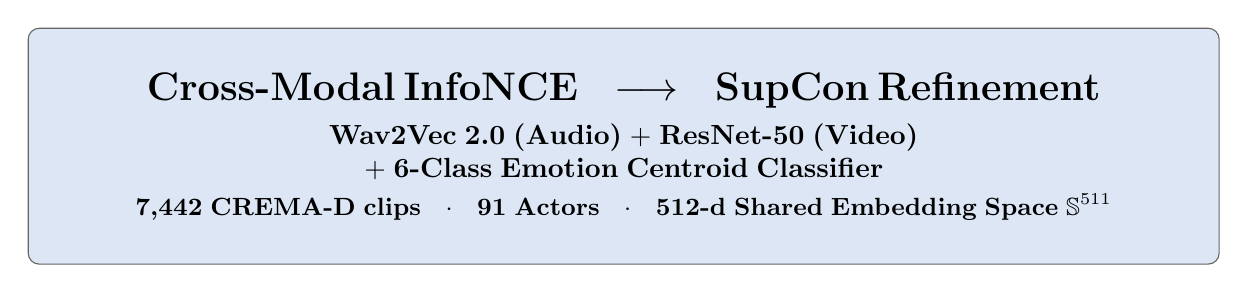
\begin{tikzpicture}
  \node[basebox, fill=cBlue, text width=14cm, inner sep=16pt]{
    \Large\bfseries Cross-Modal InfoNCE $\;\longrightarrow\;$ SupCon Refinement\\[4pt]
    \normalsize Wav2Vec 2.0 (Audio) $+$ ResNet-50 (Video) $+$
    6-Class Emotion Centroid Classifier\\[4pt]
    \small 7,442 CREMA-D clips $\;\cdot\;$ 91 Actors $\;\cdot\;$
    512-d Shared Embedding Space $\mathbb{S}^{511}$
  };
\end{tikzpicture}

\vspace{1.5cm}

{\large\bfseries IT 581 Project — Technical Documentation}\\[0.3cm]
{\large Oluwakayode Soyinka}\\[0.2cm]
{\normalsize MIVA-KNIGHT: Multimodal Intelligent Voice Assistant — Knight}\\[1.0cm]

\begin{tabular}{ll}
\toprule
\textbf{Document Type}  & Standalone Technical Report + Algorithm Reference \\
\textbf{Notebook}       & MIVA\_KNIGHT\_PipelineD\_CREMAD\_Annotated.ipynb \\
\textbf{Pipeline}       & D (final pipeline of 4) \\
\textbf{Dataset}        & CREMA-D (7,442 clips, 91 actors, 6 emotions) \\
\textbf{Backbone 1}     & Wav2Vec 2.0 — \texttt{facebook/wav2vec2-base-960h} \\
\textbf{Backbone 2}     & ResNet-50 (ImageNet pretrained) \\
\textbf{Training Mode}  & Cross-modal InfoNCE (Stage 1) + SupCon (Stage 2) \\
\textbf{Embed Dim}      & 512 (shared across all 4 pipelines) \\
\bottomrule
\end{tabular}

\vfill
{\small\color{gray} This document explains every algorithm, architecture decision,
mathematical formulation, and design choice in Pipeline D.\\
Both technical derivations and plain-language explanations are provided throughout.}
\end{titlepage}

\tableofcontents
\newpage

% ═══════════════════════════════════════════════════
\section{System Overview and Motivation}
% ═══════════════════════════════════════════════════

\subsection{What is MIVA-KNIGHT?}

MIVA-KNIGHT (\textbf{M}ultimodal \textbf{I}ntelligent \textbf{V}oice
\textbf{A}ssistant — \textbf{KNIGHT}) is a four-pipeline deep learning system
that learns to embed text, images, audio, and video into a single shared
512-dimensional space. The end goal is a voice assistant that can:
\begin{enumerate}
  \item Answer general-domain questions (Pipeline A — COCO text+image)
  \item Answer medical-domain questions (Pipeline B — ROCO medical text+image)
  \item Detect the emotional tone of the user's speech (Pipeline C — RAVDESS audio)
  \item Perform richer audio-visual emotion recognition (Pipeline D — CREMA-D)
\end{enumerate}

\begin{remark}[Plain-language summary]
Think of MIVA-KNIGHT as a voice assistant that has been trained in four
school subjects. Pipeline D is its final exam subject: watching short video
clips of people speaking, simultaneously processing both their voice and their
face, and deciding what emotion they are expressing. Once trained, the assistant
can detect whether you sound angry, happy, sad, and so on — and then tailor
its responses accordingly.
\end{remark}

\subsection{Pipeline D in Context}

\begin{table}[H]
\centering
\caption{The four MIVA-KNIGHT pipelines}
\begin{tabularx}{\textwidth}{lXXXX}
\toprule
& \textbf{Pipeline A} & \textbf{Pipeline B} & \textbf{Pipeline C} & \textbf{Pipeline D} \\
\midrule
Dataset      & COCO           & ROCO           & RAVDESS         & CREMA-D \\
Modalities   & Text + Image   & Med.\ Text + Image & Audio only  & Audio + Video \\
Loss         & InfoNCE        & InfoNCE        & SupCon          & InfoNCE $\to$ SupCon \\
Epochs       & 15             & Fine-tune      & 30              & 13 + 10 \\
Result       & P@1 = 64.6\%   & MRR = 0.727    & 6/8 @ 59.0\%    & TBD \\
\bottomrule
\end{tabularx}
\end{table}

\subsection{Key Design Decisions in Pipeline D}

\begin{enumerate}
  \item \textbf{Two frozen backbones.} Wav2Vec 2.0 (94 M params) and ResNet-50
        (23 M params) extract features once and save them to disk. Only the
        lightweight projection heads ($\approx$3.6 M trainable params) are
        updated during training.
  \item \textbf{Two-stage contrastive training.} Stage 1 (InfoNCE) aligns audio
        and video embeddings using the natural pairing signal of clips. Stage 2
        (SupCon) sharpens emotion-class cluster boundaries using explicit labels.
  \item \textbf{Warm-start from Pipeline C.} AudioProjection weights from
        RAVDESS training are inherited, giving Pipeline D a head-start on
        6 shared emotion classes.
  \item \textbf{Shared embedding space $\mathbb{S}^{511}$.} All four pipelines
        map their modality to the same 512-d unit hypersphere, enabling
        cross-pipeline cosine-similarity comparisons.
\end{enumerate}

% ═══════════════════════════════════════════════════
\section{Full Pipeline Flowchart}
% ═══════════════════════════════════════════════════

Figure~\ref{fig:pipeline_flowchart} shows the complete Pipeline D data-flow
from raw CREMA-D \texttt{.mp4} clips through feature extraction, projection,
contrastive training, and final inference.

\begin{figure}[H]
\centering
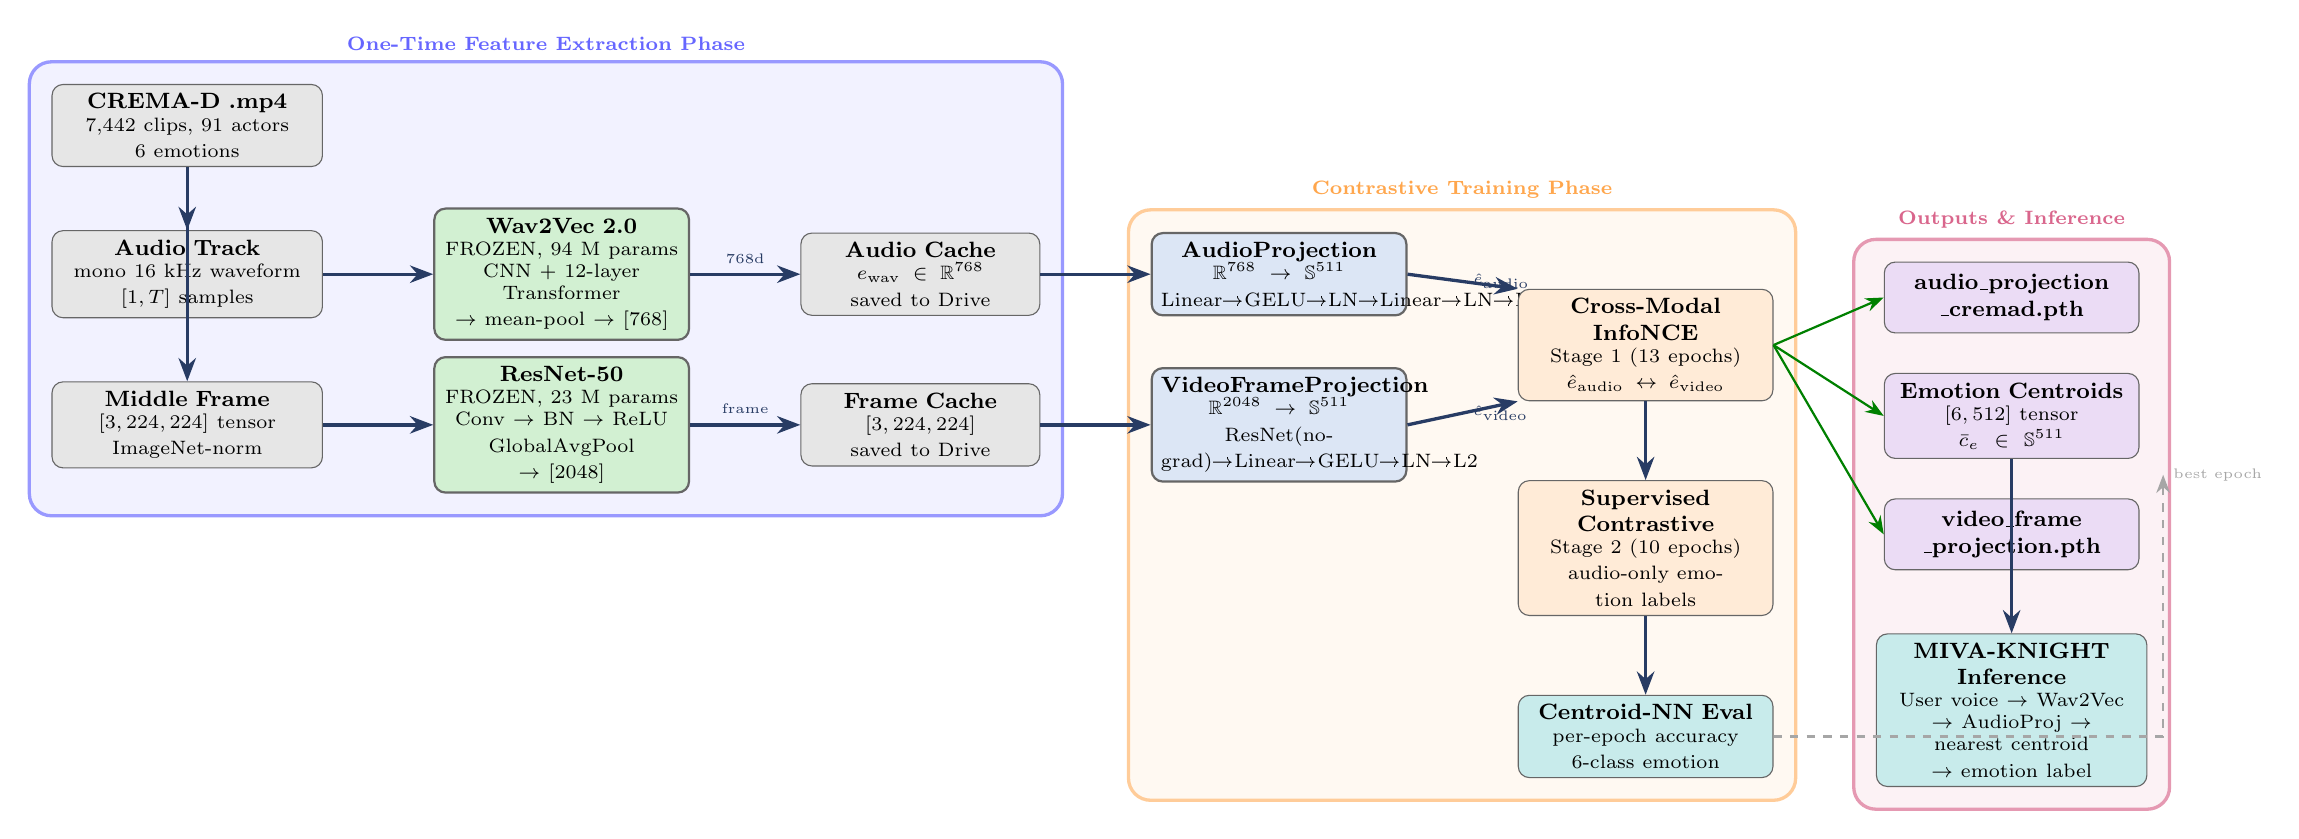
\begin{tikzpicture}[node distance=0.9cm and 1.2cm]

  % ── Column 1: DATA ──
  \node[datanode, text width=3.2cm] (mp4)
      {\textbf{CREMA-D .mp4}\\\scriptsize 7,442 clips, 91 actors\\6 emotions};

  \node[datanode, text width=3.2cm, below=0.8cm of mp4] (audio_raw)
      {\textbf{Audio Track}\\\scriptsize mono 16 kHz waveform\\$[1, T]$ samples};

  \node[datanode, text width=3.2cm, below=0.8cm of audio_raw] (video_raw)
      {\textbf{Middle Frame}\\\scriptsize $[3,224,224]$ tensor\\ImageNet-norm};

  % ── Column 2: BACKBONES (frozen) ──
  \node[modelnode, text width=3.0cm, right=1.4cm of audio_raw] (wav2vec)
      {\textbf{Wav2Vec 2.0}\\\scriptsize FROZEN, 94 M params\\CNN + 12-layer Transformer\\
       \scriptsize $\to$ mean-pool $\to$ $[768]$};

  \node[modelnode, text width=3.0cm, right=1.4cm of video_raw] (resnet)
      {\textbf{ResNet-50}\\\scriptsize FROZEN, 23 M params\\Conv $\to$ BN $\to$ ReLU\\
       \scriptsize GlobalAvgPool $\to$ $[2048]$};

  % ── Column 3: CACHE ──
  \node[datanode, text width=2.8cm, right=1.4cm of wav2vec] (cache_a)
      {\textbf{Audio Cache}\\\scriptsize $e_{\text{wav}} \in \mathbb{R}^{768}$\\saved to Drive};

  \node[datanode, text width=2.8cm, right=1.4cm of resnet] (cache_v)
      {\textbf{Frame Cache}\\\scriptsize $[3,224,224]$\\saved to Drive};

  % ── Column 4: PROJECTION HEADS ──
  \node[pipenode, text width=3.0cm, right=1.4cm of cache_a] (audioproj)
      {\textbf{AudioProjection}\\\scriptsize $\mathbb{R}^{768} \to \mathbb{S}^{511}$\\
       \scriptsize Linear→GELU→LN→Linear→LN→L2};

  \node[pipenode, text width=3.0cm, right=1.4cm of cache_v] (videoproj)
      {\textbf{VideoFrameProjection}\\\scriptsize $\mathbb{R}^{2048} \to \mathbb{S}^{511}$\\
       \scriptsize ResNet(no-grad)→Linear→GELU→LN→L2};

  % ── Column 5: LOSS ──
  \node[lossnode, text width=3.0cm, right=1.4cm of audioproj, yshift=-0.9cm] (infonce)
      {\textbf{Cross-Modal InfoNCE}\\\scriptsize Stage 1 (13 epochs)\\
       \scriptsize $\hat{e}_{\text{audio}} \leftrightarrow \hat{e}_{\text{video}}$};

  % ── Stage 2 ──
  \node[lossnode, text width=3.0cm, below=1.0cm of infonce] (supcon)
      {\textbf{Supervised Contrastive}\\\scriptsize Stage 2 (10 epochs)\\
       \scriptsize audio-only emotion labels};

  % ── Evaluation ──
  \node[infernode, text width=3.0cm, below=1.0cm of supcon] (eval)
      {\textbf{Centroid-NN Eval}\\\scriptsize per-epoch accuracy\\6-class emotion};

  % ── Outputs ──
  \node[outputnode, text width=3.0cm, right=1.4cm of infonce, yshift=-0.9cm] (centroids)
      {\textbf{Emotion Centroids}\\\scriptsize $[6,512]$ tensor\\$\bar{c}_e \in \mathbb{S}^{511}$};

  \node[outputnode, text width=3.0cm, above=0.5cm of centroids] (ckpt_a)
      {\textbf{audio\_projection\\\_cremad.pth}};

  \node[outputnode, text width=3.0cm, below=0.5cm of centroids] (ckpt_v)
      {\textbf{video\_frame\\\_projection.pth}};

  % ── Inference box ──
  \node[infernode, text width=3.2cm, below=0.8cm of ckpt_v] (inference)
      {\textbf{MIVA-KNIGHT\\Inference}\\\scriptsize User voice $\to$ Wav2Vec\\
       $\to$ AudioProj $\to$ nearest centroid\\$\to$ emotion label};

  % ── ARROWS ──
  \draw[thickarrow] (mp4.south) -- (audio_raw.north);
  \draw[thickarrow] (mp4.south) -- ++(0,-0.4) -| (video_raw.north);
  \draw[thickarrow] (audio_raw.east) -- (wav2vec.west);
  \draw[thickarrow] (video_raw.east) -- (resnet.west);
  \draw[thickarrow] (wav2vec.east) -- node[above,font=\tiny]{768d} (cache_a.west);
  \draw[thickarrow] (resnet.east) -- node[above,font=\tiny]{frame} (cache_v.west);
  \draw[thickarrow] (cache_a.east) -- (audioproj.west);
  \draw[thickarrow] (cache_v.east) -- (videoproj.west);
  \draw[thickarrow] (audioproj.east) -- node[right,font=\tiny]{$\hat{e}_{\text{audio}}$} (infonce.north west);
  \draw[thickarrow] (videoproj.east) -- node[right,font=\tiny]{$\hat{e}_{\text{video}}$} (infonce.south west);
  \draw[thickarrow] (infonce.south) -- (supcon.north);
  \draw[thickarrow] (supcon.south) -- (eval.north);
  \draw[greenarrow] (infonce.east) -- (ckpt_a.west);
  \draw[greenarrow] (infonce.east) -- (centroids.west);
  \draw[greenarrow] (infonce.east) -- (ckpt_v.west);
  \draw[thickarrow] (centroids.south) -- (inference.north);
  \draw[dashedarrow] (eval.east) -| ($(centroids.south east)+(0.3,-0.2)$)
      node[right,font=\tiny]{best epoch};

  % ── Background container ──
  \begin{pgfonlayer}{background}
    \node[rectangle, draw=blue!40, fill=blue!5, very thick, rounded corners=8pt,
          fit=(mp4)(wav2vec)(resnet)(cache_a)(cache_v), inner sep=8pt,
          label={[font=\scriptsize\bfseries, text=blue!60]above:One-Time Feature Extraction Phase}] {};
    \node[rectangle, draw=orange!40, fill=orange!5, very thick, rounded corners=8pt,
          fit=(audioproj)(videoproj)(infonce)(supcon)(eval), inner sep=8pt,
          label={[font=\scriptsize\bfseries, text=orange!70]above:Contrastive Training Phase}] {};
    \node[rectangle, draw=purple!40, fill=purple!5, very thick, rounded corners=8pt,
          fit=(ckpt_a)(ckpt_v)(centroids)(inference), inner sep=8pt,
          label={[font=\scriptsize\bfseries, text=purple!60]above:Outputs \& Inference}] {};
  \end{pgfonlayer}

\end{tikzpicture}
\caption{Complete Pipeline D flowchart: from raw CREMA-D clips to trained
emotion-detection models and live inference.}
\label{fig:pipeline_flowchart}
\end{figure}

% ═══════════════════════════════════════════════════
\section{Dataset: CREMA-D}
% ═══════════════════════════════════════════════════

\subsection{Dataset Description}

CREMA-D (Crowd-Sourced Emotional Multimodal Actors Dataset) contains 7,442
short video clips of 91 actors (48 male, 43 female) performing 12 sentences
in 6 emotion categories at 4 emotional intensity levels.

\subsection{Filename Encoding}

Every clip encodes its metadata directly in the filename:

\begin{center}
\texttt{1001 \_ DFA \_ ANG \_ XX .mp4}
\end{center}
\begin{center}
\begin{tabular}{ll}
\toprule
Part & Meaning \\
\midrule
\texttt{1001}  & Actor ID (1001–1091, i.e., 91 actors) \\
\texttt{DFA}   & Sentence code (12 standardised sentences) \\
\texttt{ANG}   & Emotion code (3-letter abbreviation) \\
\texttt{XX}    & Intensity level (Lo, Med, Hi, XX = unspecified) \\
\bottomrule
\end{tabular}
\end{center}

\subsection{Emotion Label Mapping}

\begin{table}[H]
\centering
\caption{CREMA-D 6-class emotion mapping}
\begin{tabular}{ccc}
\toprule
\textbf{Filename Code} & \textbf{Emotion} & \textbf{Integer Label} \\
\midrule
\texttt{ANG} & angry   & 0 \\
\texttt{DIS} & disgust & 1 \\
\texttt{FEA} & fearful & 2 \\
\texttt{HAP} & happy   & 3 \\
\texttt{NEU} & neutral & 4 \\
\texttt{SAD} & sad     & 5 \\
\bottomrule
\end{tabular}
\end{table}

% ═══════════════════════════════════════════════════
\section{Algorithms: Data Preprocessing}
% ═══════════════════════════════════════════════════

\subsection{Filename Parser}

\begin{algorithm}[H]
\caption{CREMA-D Filename Parser}
\label{alg:filename_parser}
\begin{algorithmic}[1]
\Require \texttt{filename}: string, e.g.\ \texttt{"1001\_DFA\_ANG\_XX.mp4"}
\Ensure Metadata dictionary or \textbf{None}
\State $\textit{stem} \gets \textsc{StripExtension}(\textsc{Basename}(\textit{filename}))$
\State $\textit{parts} \gets \textit{stem}.\textsc{Split}(\texttt{'\_'})$
\If{$|\textit{parts}| \notin \{4, 5\}$}
  \State \Return \textbf{None} \Comment{Malformed filename}
\EndIf
\State $\textit{actor\_str} \gets \textit{parts}[0]$; \quad
       $\textit{sentence} \gets \textit{parts}[1]$; \quad
       $\textit{emo\_code} \gets \textit{parts}[2]$
\If{$\textit{emo\_code} \notin \textsc{CREMA\_EMOTION\_MAP}$}
  \State \Return \textbf{None} \Comment{Unknown emotion code}
\EndIf
\State $\textit{actor\_id} \gets \textsc{Int}(\textit{actor\_str})$ \Comment{Exception $\Rightarrow$ return \textbf{None}}
\State \Return $\bigl\{\texttt{actor\_id}: \textit{actor\_id},\;
               \texttt{sentence}: \textit{sentence},\;
               \texttt{emotion}: \textsc{CREMA\_EMOTION\_MAP}[\textit{emo\_code}],\;
               \texttt{stem}: \textit{stem}\bigr\}$
\end{algorithmic}
\end{algorithm}

\begin{remark}[Plain-language]
The parser is like reading a standardised library call number.
Every CREMA-D filename is a structured code: the first four characters identify
the actor, then the sentence spoken, then the emotion, then the intensity.
The parser reads this code and extracts the emotion label needed for training.
\end{remark}

\subsection{Middle-Frame Extraction}

\begin{theorem}[Peak Expression Frame]
The middle frame of a short acted-emotion clip ($\leq 3$\,s) statistically
maximises the probability of capturing the peak facial action unit configuration
for that emotion category, as actors complete their ramp-up phase in the first
half of the clip and begin relaxation in the final quarter.
\end{theorem}

\begin{algorithm}[H]
\caption{Middle-Frame Extraction from .mp4}
\label{alg:frame_extract}
\begin{algorithmic}[1]
\Require \texttt{mp4\_path}: path to video file
\Ensure $(f, \textit{success})$ where $f \in \mathbb{R}^{3 \times 224 \times 224}$
\If{\texttt{cv2} not available}
  \State \Return $(\textsc{GrayFrame}, \textbf{False})$ \Comment{fallback placeholder}
\EndIf
\State $\textit{cap} \gets \textsc{cv2.VideoCapture}(\textit{mp4\_path})$
\If{$\neg\,\textit{cap}.\textsc{isOpened}()$}
  \State \Return $(\textsc{GrayFrame}, \textbf{False})$
\EndIf
\State $N \gets \textit{cap}.\textsc{get}(\texttt{CAP\_PROP\_FRAME\_COUNT})$
\If{$N = 0$}
  \State \Return $(\textsc{GrayFrame}, \textbf{False})$
\EndIf
\State $\textit{cap}.\textsc{set}(\texttt{CAP\_PROP\_POS\_FRAMES},\; \max(0,\, \lfloor N/2 \rfloor))$
       \Comment{Seek to midpoint}
\State $(\textit{ret}, \textit{frame}) \gets \textit{cap}.\textsc{read}()$; \quad $\textit{cap}.\textsc{release}()$
\If{$\neg\,\textit{ret}$}
  \State \Return $(\textsc{GrayFrame}, \textbf{False})$
\EndIf
\State $\textit{rgb} \gets \textsc{cv2.cvtColor}(\textit{frame},\; \texttt{COLOR\_BGR2RGB})$
       \Comment{OpenCV is BGR; PIL needs RGB}
\State $\textit{pil} \gets \textsc{Image.fromarray}(\textit{rgb})$
\State $f \gets \textsc{FRAME\_TRANSFORM}(\textit{pil})$
       \Comment{Resize(224)$\to$CentreC$\to$ToTensor$\to$ImageNet-Norm}
\State \Return $(f, \textbf{True})$
\end{algorithmic}
\end{algorithm}

\subsubsection{ImageNet Normalisation}

\begin{definition}[ImageNet Channel Normalisation]
For a frame tensor $x \in [0,1]^{3 \times H \times W}$, channel-wise
normalisation produces:
\[
  \hat{x}_{c,h,w} = \frac{x_{c,h,w} - \mu_c}{\sigma_c}, \qquad
  \boldsymbol{\mu} = [0.485, 0.456, 0.406], \quad
  \boldsymbol{\sigma} = [0.229, 0.224, 0.225]
\]
These constants are the per-channel means and standard deviations of the
ImageNet-1k training set. Pre-trained ResNet-50 expects inputs in this
distribution; using different statistics degrades feature quality.
\end{definition}

\begin{remark}[Plain-language]
OpenCV stores images as Blue-Green-Red (BGR) but PyTorch models expect
Red-Green-Blue (RGB). After flipping the channel order, we resize the frame
to $224 \times 224$ pixels (the standard ResNet input size) and subtract
the average colour values learned from one million training images.
This ensures the frozen ResNet-50 sees inputs that look like what it was
trained on.
\end{remark}

% ═══════════════════════════════════════════════════
\section{Backbone Architecture: Wav2Vec 2.0}
% ═══════════════════════════════════════════════════

\subsection{Architecture Overview}

\begin{axiom}[Self-Supervised Speech Representations]
A model trained on 960 hours of unlabelled speech (LibriSpeech) to solve a
masked contrastive prediction task learns richer phonemic and prosodic
representations than any model trained only on labelled emotion data, because
the scale of unsupervised data ($> 10^6$ utterances) far exceeds the scale
of any emotion dataset ($< 10^4$ clips).
\end{axiom}

Wav2Vec 2.0 (Baevski et al., NeurIPS 2020) processes raw waveforms:

\[
\text{Raw waveform} \in \mathbb{R}^{T}
  \xrightarrow{\text{CNN encoder}(7\text{ layers})}
  \mathbb{R}^{T' \times 512}
  \xrightarrow{\text{Transformer}(12\text{ layers}, d=768)}
  \mathbb{R}^{T' \times 768}
  \xrightarrow{\text{mean-pool}}
  \mathbb{R}^{768}
\]

where $T' \approx T/320$ (one context frame per 20\,ms at 16\,kHz).

\subsection{Mean-Pooling Justification}

\begin{theorem}[Global Emotion Pooling]
For a clip of duration $D$ seconds at sample rate $f_s = 16{,}000$\,Hz,
let $h_t^{(L)} \in \mathbb{R}^{768}$ be the $L$-th Transformer layer
output at frame $t$. The sentence-level audio embedding is:
\[
  e_{\text{wav}} = \frac{1}{T'}\sum_{t=1}^{T'} h_t^{(L)} \in \mathbb{R}^{768}
\]
This is the minimum-variance unbiased estimator of the clip's
mean emotional state under the assumption that emotion is a stationary
global property of the utterance (not localised to a single frame).
\end{theorem}

\begin{proof}[Sketch]
Let $h_t = \mu_e + \epsilon_t$ where $\mu_e$ is the true emotion embedding
and $\epsilon_t \sim \mathcal{N}(0, \sigma^2 I)$ is per-frame noise.
By linearity of expectation, $\mathbb{E}[\bar{h}] = \mu_e$ (unbiased).
Variance: $\mathrm{Var}(\bar{h}) = \sigma^2/T'$ — decreasing in $T'$, so
longer clips yield lower-variance estimates of $\mu_e$.\qed
\end{proof}

\subsection{Audio Preprocessing Pipeline}

\begin{algorithm}[H]
\caption{Audio Preprocessing for Wav2Vec 2.0}
\label{alg:audio_preproc}
\begin{algorithmic}[1]
\Require \texttt{mp4\_path}: video file path
\Ensure $e_{\text{wav}} \in \mathbb{R}^{768}$ or \textbf{None} on failure
\State $(\textit{waveform}, \textit{sr}) \gets \textsc{torchaudio.load}(\textit{mp4\_path})$
       \Comment{$[C, T]$}
\If{$\textit{sr} \neq 16000$}
  \State $\textit{waveform} \gets \textsc{Resample}(\textit{waveform}, \textit{sr}, 16000)$
\EndIf
\If{$\textit{waveform.shape}[0] > 1$}
  \State $\textit{waveform} \gets \textit{waveform}.\textsc{mean}(\text{dim}=0, \text{keepdim}=\text{True})$
         \Comment{Stereo $\to$ Mono}
\EndIf
\State $\textit{inp} \gets \textit{waveform}.\textsc{squeeze}(0).\textsc{numpy}()$
       \Comment{$[T]$ float32}
\State $\textit{input\_values} \gets \textsc{Wav2Vec2Processor}(\textit{inp}, \text{sr}=16000)$
\State \textbf{with} \texttt{torch.no\_grad():}
\State $\quad \textit{out} \gets \textsc{Wav2Vec2Model}(\textit{input\_values}).\texttt{last\_hidden\_state}$
       \Comment{$[1, T', 768]$}
\State $\textit{e\_wav} \gets \textit{out}.\textsc{mean}(\text{dim}=1).\textsc{cpu}()$
       \Comment{$[1, 768]$}
\State \Return $\textit{e\_wav}$
\end{algorithmic}
\end{algorithm}

% ═══════════════════════════════════════════════════
\section{Feature Caching Algorithm}
% ═══════════════════════════════════════════════════

\subsection{Motivation: Caching Speed-up}

\begin{lemma}[Caching Efficiency]
\label{lem:cache_speedup}
Let $t_{\text{fwd}}$ be the Wav2Vec forward-pass time per clip and $E$ the
number of training epochs. Without caching:
\[
  T_{\text{no-cache}} = N \cdot E \cdot t_{\text{fwd}} = 7{,}442 \times 13 \times 0.3\,\text{s}
  \approx 29{,}024\,\text{s} \approx 8\,\text{hours}
\]
With one-time caching ($T_{\text{extract}} \approx 1{,}080$\,s) and per-epoch
cache-read time $T_e \approx 30$\,s:
\[
  T_{\text{cached}} \approx T_{\text{extract}} + E \cdot T_e
  = 1{,}080 + 13 \times 30 \approx 1{,}470\,\text{s} \approx 27\,\text{min}
\]
Speed-up factor: $T_{\text{no-cache}}/T_{\text{cached}} \approx \mathbf{20\times}$.
\end{lemma}

\subsection{Full Extraction and Cache Algorithm}

\begin{algorithm}[H]
\caption{One-Time Feature Extraction and Cache}
\label{alg:cache}
\begin{algorithmic}[1]
\Require $\textit{all\_mp4}$: list of $(\textit{path}, \textit{meta})$ tuples;
         $\textsc{CACHE\_FILE}$: Drive path
\Ensure $\textit{cache}$: dict mapping stem $\to$ features
\If{$\textsc{CacheFile.exists}()$ \textbf{and} $|\textit{cache}| > 100$}
  \State $\textit{cache} \gets \textsc{torch.load}(\textsc{CACHE\_FILE})$
  \State \textbf{assert} $\textit{cache}[*][\texttt{'audio\_emb'}].\text{shape}[0] = 768$
         \Comment{Dimension guard}
  \State \Return $\textit{cache}$ \Comment{Resume-safe shortcut}
\EndIf
\State $\textit{wav2vec} \gets \textsc{Wav2VecEncoder}().\textsc{to}(\textit{device})$
\ForEach{$(\textit{path}, \textit{meta}) \in \textit{all\_mp4}$}
  \State $\textit{audio\_emb} \gets \textsc{Wav2VecEncode}(\textit{path})$
         \Comment{$\in \mathbb{R}^{768}$; skip on exception}
  \State $(\textit{frame}, \textit{ok}) \gets \textsc{ExtractMiddleFrame}(\textit{path})$
         \Comment{$\in \mathbb{R}^{3\times224\times224}$}
  \State $\textit{cache}[\textit{meta}[\texttt{stem}]] \gets \{$
  \State $\quad \texttt{audio\_emb}: \textit{audio\_emb},\quad
               \texttt{frame\_tensor}: \textit{frame},$
  \State $\quad \texttt{emotion}: \textit{meta}[\texttt{emotion}],\quad
               \texttt{label}: \textsc{EmotionToLabel}[\textit{meta}[\texttt{emotion}]],$
  \State $\quad \texttt{actor\_id}: \textit{meta}[\texttt{actor\_id}],\quad
               \texttt{has\_video}: \textit{ok}\;\}$
\EndFor
\State \textbf{del} $\textit{wav2vec}$; $\textsc{torch.cuda.empty\_cache}()$
       \Comment{Free 360 MB VRAM}
\State $\textsc{torch.save}(\textit{cache}, \textsc{CACHE\_FILE})$
\State $n_V \gets \sum \textit{cache}[*][\texttt{has\_video}]$
\State $\textsc{CROSS\_MODAL} \gets (n_V / |\textit{cache}|) \geq 0.5$
       \Comment{Fallback to SupCon if $< 50\%$ clips have video}
\State \Return $\textit{cache}$
\end{algorithmic}
\end{algorithm}

\begin{remark}[VRAM Lifecycle]
Wav2Vec occupies $\approx$360 MB of VRAM during extraction. After
\texttt{del wav2vec} and \texttt{torch.cuda.empty\_cache()}, that memory
is returned to the GPU allocator before the projection heads are loaded.
This prevents out-of-memory (OOM) errors on the 16 GB Colab T4.
\end{remark}

% ═══════════════════════════════════════════════════
\section{Neural Network Architectures}
% ═══════════════════════════════════════════════════

\subsection{AudioProjection Head}

\subsubsection{Formal Definition}

\begin{definition}[AudioProjection]
Let $x \in \mathbb{R}^{768}$ be the Wav2Vec mean-pooled embedding.
The AudioProjection maps:
\[
  f_\theta^{\text{audio}} : \mathbb{R}^{768} \to \mathbb{S}^{511}, \qquad
  f_\theta^{\text{audio}}(x) = \frac{g_\theta(x)}{\|g_\theta(x)\|_2}
\]
where the pre-normalisation map is:
\[
  g_\theta(x) = \text{LN}_{512}\!\Bigl(W_2 \cdot \text{GELU}\bigl(\text{LN}_{768}(W_1 x + b_1)\bigr) + b_2\Bigr)
\]
with $W_1 \in \mathbb{R}^{768 \times 768}$, $W_2 \in \mathbb{R}^{512 \times 768}$.
\end{definition}

\subsubsection{Architecture Diagram}

\begin{figure}[H]
\centering
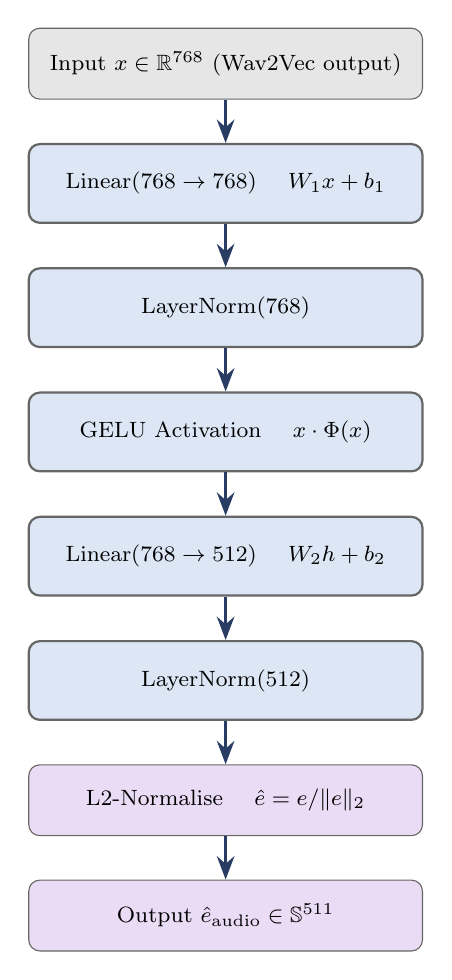
\begin{tikzpicture}[node distance=0.55cm]
  \node[datanode, minimum width=5cm] (inp) {Input $x \in \mathbb{R}^{768}$ (Wav2Vec output)};
  \node[pipenode, minimum width=5cm, below=of inp] (l1)
      {Linear$(768 \to 768)$ \quad $W_1 x + b_1$};
  \node[pipenode, minimum width=5cm, below=of l1] (ln1)
      {LayerNorm$(768)$};
  \node[pipenode, minimum width=5cm, below=of ln1] (gelu)
      {GELU Activation \quad $x \cdot \Phi(x)$};
  \node[pipenode, minimum width=5cm, below=of gelu] (l2)
      {Linear$(768 \to 512)$ \quad $W_2 h + b_2$};
  \node[pipenode, minimum width=5cm, below=of l2] (ln2)
      {LayerNorm$(512)$};
  \node[outputnode, minimum width=5cm, below=of ln2] (l2norm)
      {L2-Normalise \quad $\hat{e} = e / \|e\|_2$};
  \node[outputnode, minimum width=5cm, below=of l2norm] (out)
      {Output $\hat{e}_{\text{audio}} \in \mathbb{S}^{511}$};

  \foreach \from/\to in {inp/l1, l1/ln1, ln1/gelu, gelu/l2, l2/ln2, ln2/l2norm, l2norm/out}
    \draw[thickarrow] (\from) -- (\to);
\end{tikzpicture}
\caption{AudioProjection head architecture.}
\end{figure}

\subsubsection{Parameter Count}

\begin{table}[H]
\centering
\caption{AudioProjection trainable parameters}
\begin{tabular}{lrc}
\toprule
Layer & Parameters & Formula \\
\midrule
Linear$(768 \to 768)$ & 590,592 & $768^2 + 768$ \\
LayerNorm$(768)$       & 1,536   & $2 \times 768$ \\
Linear$(768 \to 512)$ & 393,728 & $768 \times 512 + 512$ \\
LayerNorm$(512)$       & 1,024   & $2 \times 512$ \\
\midrule
\textbf{Total}         & \textbf{986,880} & \\
\bottomrule
\end{tabular}
\end{table}

\subsection{VideoFrameProjection Head}

\begin{definition}[VideoFrameProjection]
Let $I \in \mathbb{R}^{3 \times 224 \times 224}$ be an ImageNet-normalised
middle frame. ResNet-50 extracts pool5 features (frozen, inside
\texttt{torch.no\_grad()}); the trainable projection then maps:
\[
  f_\phi^{\text{video}} : \mathbb{R}^{3 \times 224 \times 224} \to \mathbb{S}^{511}
\]
\[
  f_\phi^{\text{video}}(I) = \text{L2-norm}\!\Bigl(\text{LN}_{512}\Bigl(
    W_4 \cdot \text{GELU}\bigl(\text{LN}_{1024}(W_3 \cdot r(I) + b_3)\bigr) + b_4
  \Bigr)\Bigr)
\]
where $r(I) = \text{ResNet50}(I) \in \mathbb{R}^{2048}$ (frozen),
$W_3 \in \mathbb{R}^{1024 \times 2048}$, $W_4 \in \mathbb{R}^{512 \times 1024}$.
\end{definition}

\begin{table}[H]
\centering
\caption{VideoFrameProjection trainable parameters (backbone excluded)}
\begin{tabular}{lrc}
\toprule
Layer & Parameters & Formula \\
\midrule
Linear$(2048 \to 1024)$ & 2,098,176 & $2048 \times 1024 + 1024$ \\
LayerNorm$(1024)$        & 2,048     & $2 \times 1024$ \\
Linear$(1024 \to 512)$  & 524,800   & $1024 \times 512 + 512$ \\
LayerNorm$(512)$         & 1,024     & $2 \times 512$ \\
\midrule
\textbf{Trainable total} & \textbf{2,627,048} & \\
ResNet-50 backbone       & $\approx$23.5 M & frozen \\
\bottomrule
\end{tabular}
\end{table}

\subsection{Why Symmetric Projection Heads?}

\begin{axiom}[Common Embedding Space]
For cross-modal cosine similarity to be a meaningful distance metric,
both modalities must be embedded on the same metric space. The unit
hypersphere $\mathbb{S}^{511}$ with cosine distance satisfies the
metric axioms (non-negativity, symmetry, triangle inequality) when
all vectors are L2-normalised. Using different output norms or
embedding spaces for audio vs.\ video would violate symmetry.
\end{axiom}

% ═══════════════════════════════════════════════════
\section{Loss Functions}
% ═══════════════════════════════════════════════════

\subsection{Stage 1: Cross-Modal InfoNCE Loss}

\subsubsection{Intuition and Definition}

\begin{definition}[Cross-Modal InfoNCE Loss]
For a batch of $B$ audio-video pairs $(a_i, v_i)$, let
$S_{ij} = \hat{e}_i^{\text{audio}} \cdot \hat{e}_j^{\text{video}}$
(cosine similarity of L2-normalised embeddings). The symmetric
InfoNCE loss is:
\[
  \mathcal{L}_{\text{InfoNCE}} = \frac{1}{2}
  \left[
    -\frac{1}{B}\sum_{i=1}^{B}\log\frac{\exp(S_{ii}/\tau)}{\sum_{j=1}^{B}\exp(S_{ij}/\tau)}
    -\frac{1}{B}\sum_{j=1}^{B}\log\frac{\exp(S_{jj}/\tau)}{\sum_{i=1}^{B}\exp(S_{ij}/\tau)}
  \right]
\]
where $\tau = 0.07$ is the temperature hyperparameter.
\end{definition}

\begin{theorem}[InfoNCE Lower Bound on Mutual Information]
Maximising $-\mathcal{L}_{\text{InfoNCE}}$ is equivalent to maximising
a lower bound on the mutual information $I(A; V)$ between the audio and
video representations. Specifically:
\[
  I(A; V) \geq \log(B) - \mathcal{L}_{\text{InfoNCE}}
\]
Thus the random baseline (untrained representations) gives
$\mathcal{L}_{\text{InfoNCE}}^{\text{random}} = \log(B) = \log(32) \approx 3.47$.
\end{theorem}

\subsubsection{Algorithm}

\begin{algorithm}[H]
\caption{Cross-Modal InfoNCE Loss}
\label{alg:infonce}
\begin{algorithmic}[1]
\Require $\hat{e}^{\text{audio}} \in \mathbb{R}^{B \times 512}$,
         $\hat{e}^{\text{video}} \in \mathbb{R}^{B \times 512}$, temperature $\tau$
\Ensure $\mathcal{L}_{\text{InfoNCE}} \in \mathbb{R}$
\State $S \gets \hat{e}^{\text{audio}} \cdot (\hat{e}^{\text{video}})^\top / \tau$
       \Comment{$[B, B]$ similarity matrix}
\State $\textit{labels} \gets [0, 1, 2, \ldots, B-1]$
       \Comment{Diagonal = positive pairs}
\State $\mathcal{L}_1 \gets \textsc{CrossEntropy}(S, \textit{labels})$
       \Comment{Audio $\to$ Video direction}
\State $\mathcal{L}_2 \gets \textsc{CrossEntropy}(S^\top, \textit{labels})$
       \Comment{Video $\to$ Audio direction}
\State \Return $(\mathcal{L}_1 + \mathcal{L}_2) / 2$
\end{algorithmic}
\end{algorithm}

\begin{remark}[Plain-language]
InfoNCE works like a matching game. We show the model 32 audio clips and
32 video clips from the same 32 people. The model must match each audio clip
to its correct video (and vice versa). The score is the negative log
probability of making all 32 correct matches simultaneously.
A random guesser scores $\log(32) \approx 3.47$; a perfect matcher scores 0.
\end{remark}

\subsection{Stage 2: Supervised Contrastive Loss (SupCon)}

\subsubsection{Definition}

\begin{definition}[Supervised Contrastive Loss]
For a batch $I = \{1, \ldots, B\}$ with labels $y_i \in \{0,\ldots,5\}$,
define the positive set of anchor $i$ as
$\mathcal{P}(i) = \{p \neq i \mid y_p = y_i\}$.
The SupCon loss is:
\[
  \mathcal{L}_{\text{SupCon}} =
  \sum_{i \in I} \frac{-1}{|\mathcal{P}(i)|}
  \sum_{p \in \mathcal{P}(i)}
  \log\frac{\exp(\hat{e}_i \cdot \hat{e}_p / \tau)}
           {\sum_{a \in A(i)} \exp(\hat{e}_i \cdot \hat{e}_a / \tau)}
\]
where $A(i) = I \setminus \{i\}$ (all other samples).
\end{definition}

\begin{lemma}[SupCon Cluster Geometry]
Under SupCon minimisation, the optimal embedding geometry on
$\mathbb{S}^{511}$ concentrates each class $c$ at its normalised centroid
$\bar{c}_c = \mu_c/\|\mu_c\|_2$, with inter-class angle approaching
$\arccos(-1/(K-1))$ where $K=6$ is the number of emotion classes.
\end{lemma}

\begin{algorithm}[H]
\caption{Supervised Contrastive Loss (SupCon)}
\label{alg:supcon}
\begin{algorithmic}[1]
\Require $\hat{e} \in \mathbb{R}^{B \times 512}$ (L2-normalised),
         $y \in \mathbb{Z}^B$ (class labels), temperature $\tau$
\Ensure $\mathcal{L}_{\text{SupCon}} \in \mathbb{R}$
\State $\textit{sim} \gets \hat{e} \cdot \hat{e}^\top / \tau$
       \Comment{$[B, B]$ similarity}
\State $\textit{sim} \gets \textit{sim} - \max(\textit{sim}, \text{dim}=1)$
       \Comment{Log-sum-exp stability trick}
\State $\textit{pos\_mask} \gets (y_i = y_j)$ for $i \neq j$
       \Comment{$[B, B]$ boolean, diagonal = False}
\State $\textit{neg\_mask} \gets \neg(y_i = y_j \text{ or } i=j)$
       \Comment{Different-class pairs}
\ForEach{anchor $i$ with $|\mathcal{P}(i)| > 0$}
  \State $\textit{denom} \gets \log\sum_{a \neq i} \exp(\textit{sim}_{ia})$
  \State $\mathcal{L}_i \gets \frac{-1}{|\mathcal{P}(i)|}
    \sum_{p \in \mathcal{P}(i)} (\textit{sim}_{ip} - \textit{denom})$
\EndFor
\If{no anchors have positive pairs}
  \State \Return $\mathbf{0}$ \Comment{Zero-gradient guard}
\EndIf
\State \Return $\text{mean}(\mathcal{L}_i)$
\end{algorithmic}
\end{algorithm}

\subsubsection{InfoNCE vs SupCon Comparison}

\begin{table}[H]
\centering
\caption{InfoNCE vs SupCon: key differences}
\begin{tabularx}{\textwidth}{lXX}
\toprule
Property & InfoNCE (Stage 1) & SupCon (Stage 2) \\
\midrule
Positives per anchor & 1 (paired modality sample) & All same-class clips in batch \\
Requires second modality & Yes & No \\
Supervisory signal & Clip identity & Emotion label \\
Effect on geometry & Cross-modal alignment & Within-class compaction \\
Signal source & Self-supervised & Supervised \\
\bottomrule
\end{tabularx}
\end{table}

% ═══════════════════════════════════════════════════
\section{Dataset and DataLoader}
% ═══════════════════════════════════════════════════

\begin{algorithm}[H]
\caption{CREMADDataset Initialisation and Retrieval}
\label{alg:dataset}
\begin{algorithmic}[1]
\Require $\textit{cache}$: dict (from Algorithm~\ref{alg:cache})
\State $\textit{samples} \gets [\,]$
\ForEach{$(\textit{stem}, \textit{data}) \in \textit{cache}.\textsc{items}()$}
  \State $\textit{samples}.\textsc{append}(\{\texttt{audio\_emb}: [768],\;
    \texttt{frame\_tensor}: [3,224,224],\;\texttt{label}: \in\{0,\ldots,5\}\})$
\EndFor
\State $\textsc{\_\_getitem\_\_}(\textit{idx})$: \Return
    $(\textit{samples}[\textit{idx}][\texttt{audio\_emb}],\;
      \textit{samples}[\textit{idx}][\texttt{frame\_tensor}],\;
      \textit{samples}[\textit{idx}][\texttt{label}])$
\end{algorithmic}
\end{algorithm}

\begin{lemma}[Negative Count in InfoNCE]
With batch size $B = 32$, each anchor has $B - 1 = 31$ negatives in the
InfoNCE denominator. The random baseline accuracy is $1/B = 1/32 \approx 3.1\%$
and the random InfoNCE loss is $\log(B) = \log(32) \approx 3.47$.
\end{lemma}

% ═══════════════════════════════════════════════════
\section{Optimiser and Learning Rate Schedule}
% ═══════════════════════════════════════════════════

\subsection{AdamW Optimiser}

Only projection head parameters are passed to the optimiser—the frozen
ResNet-50 backbone is explicitly excluded:

\begin{definition}[Decoupled Weight Decay (AdamW)]
Let $\theta_t$ be parameters at step $t$, gradient $g_t$.
AdamW updates:
\begin{align*}
  m_t &= \beta_1 m_{t-1} + (1-\beta_1) g_t \\
  v_t &= \beta_2 v_{t-1} + (1-\beta_2) g_t^2 \\
  \theta_{t+1} &= \theta_t - \eta \frac{\hat{m}_t}{\sqrt{\hat{v}_t} + \epsilon}
                - \eta \lambda \theta_t
\end{align*}
where the last term is the \emph{decoupled} L2 regularisation with
$\lambda = 0.01$. Unlike L2 in Adam (which adds $\lambda g_t$ to the gradient),
AdamW applies weight decay directly to the parameters, which correctly
regularises the scale of the embedding weights.
\end{definition}

\subsection{Warmup + Cosine Decay Schedule}

\begin{definition}[Warmup-Cosine LR Schedule]
With $t_{\text{warmup}} = \lfloor t_{\text{total}} / 10 \rfloor$ steps:
\[
  \eta(t) = \begin{cases}
    \eta_0 \cdot \dfrac{t}{t_{\text{warmup}}} & t < t_{\text{warmup}} \\[8pt]
    \eta_0 \cdot \dfrac{1}{2}\!\left(1 + \cos\dfrac{\pi(t - t_{\text{warmup}})}{t_{\text{total}} - t_{\text{warmup}}}\right)
    & t \geq t_{\text{warmup}}
  \end{cases}
\]
For Pipeline D: $t_{\text{total}} = 232 \times 13 = 3{,}016$, $t_{\text{warmup}} \approx 302$.
\end{definition}

\begin{remark}[Plain-language]
The warmup phase gradually ramps up the learning rate from zero to the
full rate over the first 302 steps ($\approx$ 1.3 epochs). This prevents
large gradient updates at the start, when the randomly initialised
VideoFrameProjection head could otherwise destabilise the warm-started
AudioProjection weights. After warmup, the rate smoothly decreases via
a cosine curve to near-zero at the final step.
\end{remark}

% ═══════════════════════════════════════════════════
\section{Training Loop Algorithms}
% ═══════════════════════════════════════════════════

\subsection{Single-Epoch Training}

\begin{algorithm}[H]
\caption{Single-Epoch Training (Cross-Modal InfoNCE)}
\label{alg:train_epoch}
\begin{algorithmic}[1]
\Require epoch index, $\textit{audio\_proj}$, $\textit{video\_proj}$,
         optimiser, scheduler, data loader
\Ensure mean epoch loss $\bar{\mathcal{L}}_e$
\State $\textit{audio\_proj}.\textsc{train}()$; $\textit{video\_proj}.\textsc{train}()$
\State $\textit{losses} \gets [\,]$
\ForEach{$(\textit{audio\_batch}^{[B,768]},\; \textit{frame\_batch}^{[B,3,224,224]},\; \textit{labels}^{[B]})$ in loader}
  \State Move all tensors to GPU
  \State $\hat{e}^{\text{audio}} \gets \textit{audio\_proj}(\textit{audio\_batch})$
         \Comment{$[B,512]$, L2-normalised}
  \If{\textsc{CROSS\_MODAL}}
    \State $\hat{e}^{\text{video}} \gets \textit{video\_proj}(\textit{frame\_batch})$
           \Comment{ResNet inside \texttt{no\_grad}}
    \State $\mathcal{L} \gets \textsc{InfoNCE}(\hat{e}^{\text{audio}}, \hat{e}^{\text{video}}, \tau)$
  \Else
    \State $\mathcal{L} \gets \textsc{SupCon}(\hat{e}^{\text{audio}}, \textit{labels}, \tau)$
  \EndIf
  \State $\textit{optimiser}.\textsc{zero\_grad}()$
  \State $\mathcal{L}.\textsc{backward}()$
  \State $\textsc{ClipGradNorm}(\textit{trainable\_params}, c=1.0)$
         \Comment{$\tilde\nabla = \min(1, c/\|\nabla\|)\,\nabla$}
  \State $\textit{optimiser}.\textsc{step}()$; $\textit{scheduler}.\textsc{step}()$
  \State $\textit{losses}.\textsc{append}(\mathcal{L}.\textsc{item}())$
\EndFor
\State \Return $\text{mean}(\textit{losses})$
\end{algorithmic}
\end{algorithm}

\subsection{Gradient Clipping}

\begin{proposition}[Gradient Clipping Stability]
Clipping the $\ell_2$ norm of all trainable gradients to threshold $c=1.0$:
\[
  \tilde\nabla = \min\!\left(1,\; \frac{c}{\|\nabla\|_2}\right)\nabla
\]
prevents the VideoFrameProjection head (randomly initialised) from producing
gradient spikes that would corrupt the warm-started AudioProjection weights.
\end{proposition}

\subsection{Full Multi-Epoch Training (Stage 1)}

\begin{algorithm}[H]
\caption{Stage 1: Full Cross-Modal InfoNCE Training}
\label{alg:stage1}
\begin{algorithmic}[1]
\Require number of epochs $E = 13$
\State $(\textit{start\_epoch}, \textit{all\_losses}, \textit{all\_accs})
    \gets \textsc{LoadCheckpoint}()$
\State $\textit{best\_acc} \gets \max(\textit{all\_accs})$ if non-empty, else 0
\State $\textit{best\_audio\_sd} \gets \textbf{None}$; $\textit{best\_video\_sd} \gets \textbf{None}$
\For{$e = \textit{start\_epoch}$ \textbf{to} $E-1$}
  \State $\bar{\mathcal{L}}_e \gets \textsc{TrainEpoch}(e)$
         \Comment{Algorithm~\ref{alg:train_epoch}, $\approx 3$ min/epoch}
  \State $(\textit{acc}_e, \textit{per\_emo}_e, \_) \gets \textsc{EvaluateAccuracy}()$
         \Comment{Algorithm~\ref{alg:evaluate}, $\approx 30$\,s}
  \State $\textit{all\_losses}.\textsc{append}(\bar{\mathcal{L}}_e)$;
         $\textit{all\_accs}.\textsc{append}(\textit{acc}_e)$
  \If{$\textit{acc}_e > \textit{best\_acc}$}
    \State $\textit{best\_acc} \gets \textit{acc}_e$;
           $\hat{e} \gets e + 1$
    \State $\textit{best\_audio\_sd} \gets \textsc{DeepCopy}(\textit{audio\_proj}.\textsc{state\_dict}())$
    \State $\textit{best\_video\_sd} \gets \textsc{DeepCopy}(\textit{video\_proj}.\textsc{state\_dict}())$
  \EndIf
  \State $\textsc{SaveCheckpoint}(e, \textit{all\_losses}, \textit{all\_accs})$
\EndFor
\State Load $\textit{best\_audio\_sd}$ and $\textit{best\_video\_sd}$
\State \Return best models
\end{algorithmic}
\end{algorithm}

\subsection{Stage 2: SupCon Refinement}

\begin{algorithm}[H]
\caption{Stage 2: Supervised Contrastive Refinement}
\label{alg:stage2}
\begin{algorithmic}[1]
\Require AudioProjection (from Stage 1 best); $E_2 = 10$ epochs; $\eta_2 = 10^{-5}$
\State $\textit{supcon\_opt} \gets \textsc{AdamW}(\textit{audio\_proj.parameters}(),
    \eta_2, \lambda=0.01)$
\For{$e = 1$ \textbf{to} $E_2$}
  \State $\textit{audio\_proj}.\textsc{train}()$
  \ForEach{$(\textit{audio\_batch}, \_, \textit{labels})$ in loader}
    \State $\hat{e}^{\text{audio}} \gets \textit{audio\_proj}(\textit{audio\_batch})$
    \State $\mathcal{L} \gets \textsc{SupCon}(\hat{e}^{\text{audio}}, \textit{labels}, \tau)$
    \State $\textit{supcon\_opt}.\textsc{zero\_grad}()$
    \State $\mathcal{L}.\textsc{backward}()$
    \State $\textsc{ClipGradNorm}(\textit{audio\_proj.parameters}(), 1.0)$
    \State $\textit{supcon\_opt}.\textsc{step}()$
  \EndFor
  \State $\textit{acc}_e \gets \textsc{EvaluateAccuracy}()$
  \If{$\textit{acc}_e > \textit{best\_supcon\_acc}$}
    \State Save best Stage 2 weights
  \EndIf
\EndFor
\end{algorithmic}
\end{algorithm}

\begin{lemma}[Geometry Preservation Under Low LR]
For small perturbations $\delta\theta$ to InfoNCE-trained weights $\theta^*$:
\[
  f_{\theta^* + \delta\theta}(x) \approx f_{\theta^*}(x) + J_\theta\,\delta\theta
\]
With $\eta_2 = 10^{-5}$, the expected weight perturbation per step
$\|\delta\theta\| \approx 10^{-5} \times \|\nabla\| \approx 10^{-5} \times 0.3 = 3 \times 10^{-6}$
— small enough to preserve cross-modal InfoNCE geometry
while tightening emotion class boundaries.
\end{lemma}

% ═══════════════════════════════════════════════════
\section{Evaluation: Centroid Nearest-Neighbour Classifier}
% ═══════════════════════════════════════════════════

\subsection{Protocol}

\begin{definition}[Spherical Centroid]
For emotion class $c$ with $N_c$ projected audio embeddings
$\{\hat{a}_1^{(c)}, \ldots, \hat{a}_{N_c}^{(c)}\}$ on $\mathbb{S}^{511}$:
\[
  \bar{c}_c = \frac{\mu_c}{\|\mu_c\|_2}, \qquad
  \mu_c = \frac{1}{N_c}\sum_{i=1}^{N_c} \hat{a}_i^{(c)} \in \mathbb{R}^{512}
\]
Re-normalising $\mu_c$ returns it to the unit sphere, making it
directly comparable via cosine similarity.
\end{definition}

\begin{algorithm}[H]
\caption{Emotion Accuracy Evaluation via Centroid Nearest-Neighbour}
\label{alg:evaluate}
\begin{algorithmic}[1]
\Require $\textit{audio\_proj}$, data loader
\Ensure $\textit{acc} \in [0,1]$, per-emotion dict, centroids $[6,512]$
\State \textbf{Step 1: Project all embeddings}
\State $\textit{audio\_proj}.\textsc{eval}()$
\State $\textit{all\_embs} \gets [\,]$; $\textit{all\_labels} \gets [\,]$
\ForEach{$(\textit{audio\_batch}, \_, \textit{labels})$ in loader}
  \State $\textit{proj} \gets \textit{audio\_proj}(\textit{audio\_batch}.\textsc{to}(\textit{device})).\textsc{cpu}()$
  \State $\textit{all\_embs}.\textsc{append}(\textit{proj})$;
         $\textit{all\_labels}.\textsc{append}(\textit{labels})$
\EndFor
\State $E \gets \textsc{cat}(\textit{all\_embs})$; $Y \gets \textsc{cat}(\textit{all\_labels})$
       \Comment{$[N,512]$, $[N]$}

\State \textbf{Step 2: Compute per-class centroids}
\For{$c = 0$ \textbf{to} $5$}
  \State $\text{mask} \gets (Y = c)$
  \State $\bar{c}_c \gets \textsc{L2Norm}(E[\text{mask}].\textsc{mean}(\text{dim}=0))$
         \Comment{$[512]$ on $\mathbb{S}^{511}$}
\EndFor
\State $C \gets \textsc{stack}(\bar{c}_0, \ldots, \bar{c}_5)$
       \Comment{$[6, 512]$}

\State \textbf{Step 3: Classify}
\State $\hat{Y} \gets \arg\max(E \cdot C^\top, \text{dim}=1)$
       \Comment{$[N]$, cosine-NN}
\State $\textit{acc} \gets \text{mean}(\hat{Y} = Y)$

\State \textbf{Step 4: Per-emotion breakdown}
\For{$c = 0$ \textbf{to} $5$}
  \State $\textit{per\_emo}[\textit{EMOTIONS}[c]] \gets
    \text{mean}((\hat{Y} = Y)[(Y = c)])$
\EndFor
\State $\textit{audio\_proj}.\textsc{train}()$
\State \Return $\textit{acc}, \textit{per\_emo}, C$
\end{algorithmic}
\end{algorithm}

\subsection{Accuracy Benchmarks}

\begin{table}[H]
\centering
\caption{Accuracy interpretation for 6-class emotion classification}
\begin{tabular}{cc}
\toprule
Accuracy & Interpretation \\
\midrule
16.7\% & Random chance ($1/6$) \\
50–60\% & Broad emotion categories separating \\
66.7\% & $4/6$ emotions correct — Pipeline D target \\
83.3\% & $5/6$ emotions correct \\
100\%  & Perfect separation \\
\bottomrule
\end{tabular}
\end{table}

% ═══════════════════════════════════════════════════
\section{Emotion Centroid Computation and Voronoi Classification}
% ═══════════════════════════════════════════════════

\begin{algorithm}[H]
\caption{Compute and Save CREMA-D Emotion Centroids}
\label{alg:centroids}
\begin{algorithmic}[1]
\Require $\textit{audio\_proj}$ (best weights), data loader
\Ensure Centroid tensor $[6, 512]$ saved to \texttt{emotion\_centroids\_cremad.pt}
\State $\textit{audio\_proj}.\textsc{eval}()$
\State $\textit{emo\_embs} \gets \textsc{defaultdict}(\text{list})$
\ForEach{$(\textit{audio\_batch}, \_, \textit{labels})$ in loader}
  \State $\textit{proj} \gets \textit{audio\_proj}(\textit{audio\_batch}.\textsc{to}(\textit{device})).\textsc{cpu}()$
  \ForEach{$(\hat{e}, l) \in \textsc{zip}(\textit{proj}, \textit{labels})$}
    \State $\textit{emo\_embs}[\textsc{LABEL\_TO\_EMOTION}[l.\textsc{item}()]].\textsc{append}(\hat{e})$
  \EndFor
\EndFor
\For{$e \in \textsc{CREMA\_EMOTIONS\_6}$}
  \State $S_e \gets \textsc{stack}(\textit{emo\_embs}[e])$
         \Comment{$[N_e, 512]$}
  \State $\bar{c}_e \gets \textsc{L2Norm}(S_e.\textsc{mean}(\text{dim}=0))$
         \Comment{Spherical centroid}
\EndFor
\State $C \gets \textsc{stack}(\bar{c}_{\text{angry}}, \ldots, \bar{c}_{\text{sad}})$
       \Comment{$[6, 512]$}
\State $\textsc{torch.save}(C, \texttt{CENTROIDS\_PATH})$
\State \Return $C$
\end{algorithmic}
\end{algorithm}

\begin{definition}[Voronoi Emotion Classifier]
The centroid classifier assigns each audio embedding $\hat{e} \in \mathbb{S}^{511}$
to the nearest emotion centroid in cosine distance:
\[
  \hat{y} = \arg\max_{c \in \{0,\ldots,5\}} \hat{e} \cdot \bar{c}_c
\]
This partitions the unit sphere into 6 Voronoi cells — one per emotion.
The quality of separation is measured by the mean off-diagonal centroid similarity:
\[
  \bar{s}_{\text{off-diag}} = \frac{1}{6 \times 5}\sum_{e \neq e'} \bar{c}_e \cdot \bar{c}_{e'}
\]
Values $< 0.3$ indicate well-separated clusters; $> 0.5$ indicates insufficient
training or emotion class confusion.
\end{definition}

% ═══════════════════════════════════════════════════
\section{Warm-Start from Pipeline C}
% ═══════════════════════════════════════════════════

\begin{theorem}[Transfer Learning Benefit]
Pipeline D AudioProjection inherits weights from Pipeline C (RAVDESS training)
when the checkpoint \texttt{pipelineC/audio\_projection.pth} is available.
Because RAVDESS and CREMA-D share 6 of 8 emotion classes
(\textit{angry, disgust, fearful, happy, neutral, sad}),
the inherited weights provide a useful initial embedding geometry
for all 6 CREMA-D classes, reducing the number of InfoNCE epochs needed.
The learning rate is halved to $\eta = 5 \times 10^{-5}$ to preserve this geometry
during the first InfoNCE epochs.
\end{theorem}

\begin{remark}[Plain-language]
Imagine training to be a music teacher. Pipeline C already taught the model
to recognise emotion in RAVDESS recordings (studio actors). Rather than
starting from scratch on CREMA-D, Pipeline D inherits the same ``ear for emotion''
and continues refining it on a larger, more diverse set of 7,442 clips from 91
actors — five times more diverse than RAVDESS (24 actors).
\end{remark}

% ═══════════════════════════════════════════════════
\section{Complete Pipeline Flowchart: Training Phases}
% ═══════════════════════════════════════════════════

Figure~\ref{fig:training_phases} shows the two-stage training strategy
with warm-start inheritance and checkpoint flow.

\begin{figure}[H]
\centering
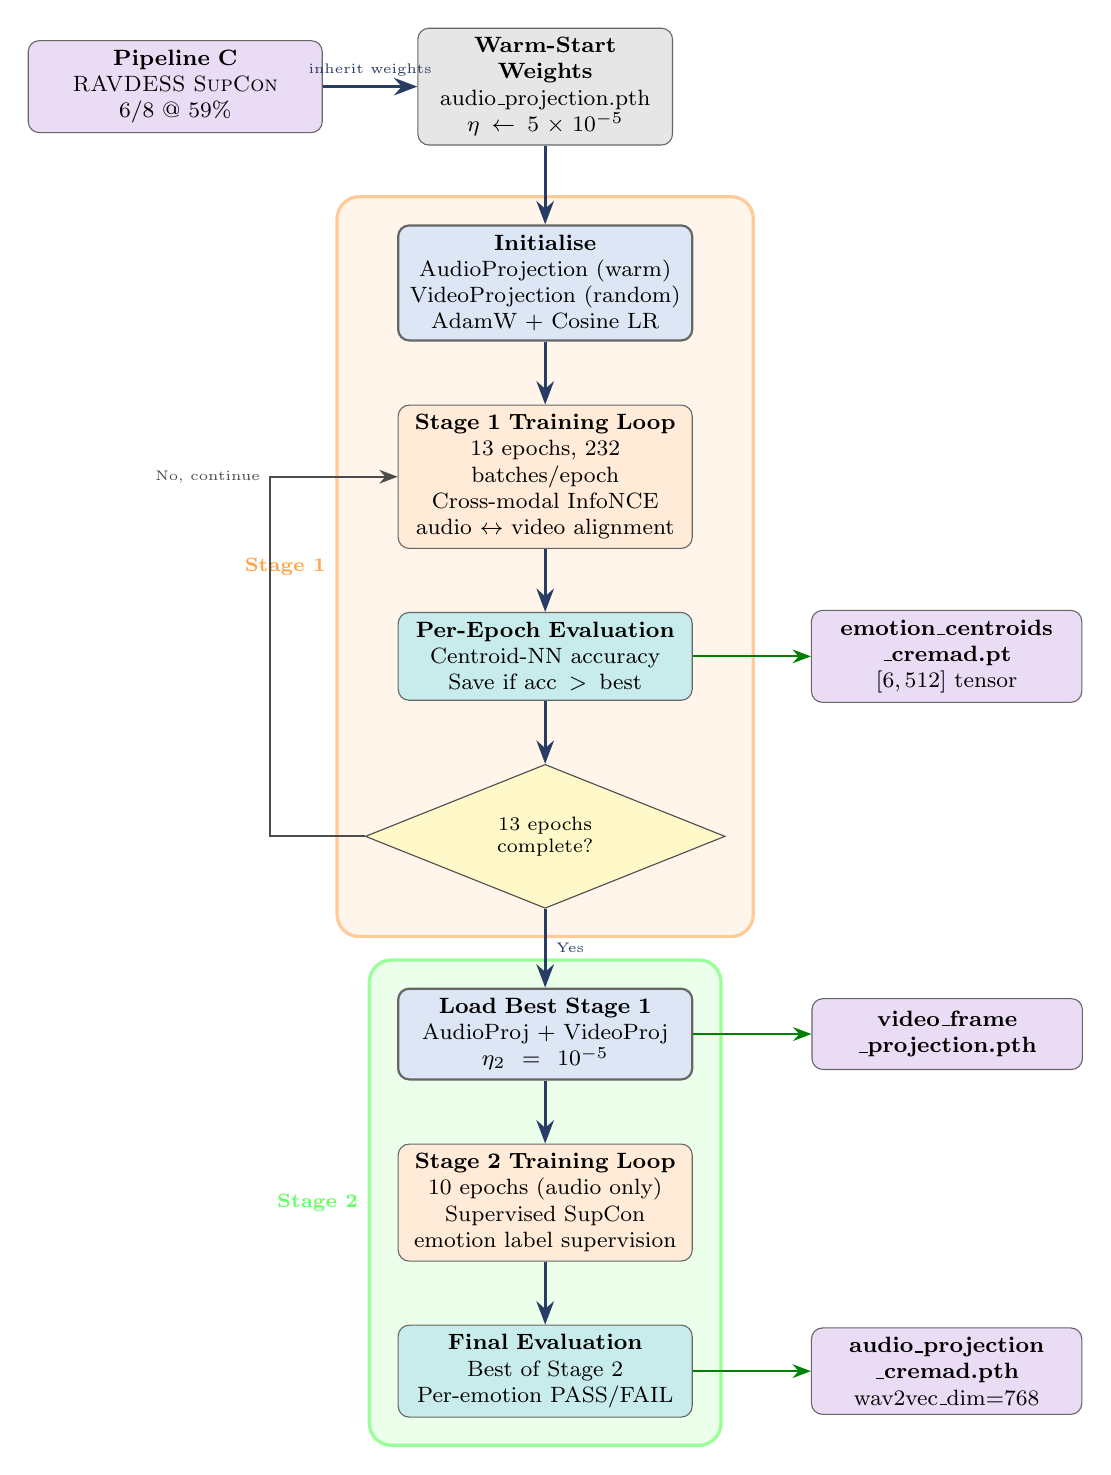
\begin{tikzpicture}[node distance=0.8cm and 1.5cm]

  % ── Pipeline C warm-start ──
  \node[outputnode, text width=3.5cm] (pipeC)
      {\textbf{Pipeline C}\\\textsc{RAVDESS SupCon}\\6/8 @ 59\%};
  \node[datanode, text width=3.0cm, right=1.2cm of pipeC] (warm)
      {\textbf{Warm-Start Weights}\\audio\_projection.pth\\$\eta \gets 5\times10^{-5}$};

  % ── Stage 1 ──
  \node[pipenode, text width=3.5cm, below=1.0cm of warm] (stage1init)
      {\textbf{Initialise}\\AudioProjection (warm)\\VideoProjection (random)\\AdamW + Cosine LR};

  \node[lossnode, text width=3.5cm, below=0.8cm of stage1init] (s1loop)
      {\textbf{Stage 1 Training Loop}\\13 epochs, 232 batches/epoch\\Cross-modal InfoNCE\\
       audio $\leftrightarrow$ video alignment};

  \node[infernode, text width=3.5cm, below=0.8cm of s1loop] (s1eval)
      {\textbf{Per-Epoch Evaluation}\\Centroid-NN accuracy\\Save if $\text{acc} > \text{best}$};

  \node[decisionnode, text width=2.5cm, below=0.8cm of s1eval]
      (s1done) {13 epochs\\complete?};

  % ── Stage 2 ──
  \node[pipenode, text width=3.5cm, below=1.0cm of s1done] (s2init)
      {\textbf{Load Best Stage 1}\\AudioProj + VideoProj\\$\eta_2 = 10^{-5}$};

  \node[lossnode, text width=3.5cm, below=0.8cm of s2init] (s2loop)
      {\textbf{Stage 2 Training Loop}\\10 epochs (audio only)\\Supervised SupCon\\
       emotion label supervision};

  \node[infernode, text width=3.5cm, below=0.8cm of s2loop] (s2eval)
      {\textbf{Final Evaluation}\\Best of Stage 2\\Per-emotion PASS/FAIL};

  % ── Outputs ──
  \node[outputnode, text width=3.2cm, right=1.5cm of s2eval] (out1)
      {\textbf{audio\_projection\\\_cremad.pth}\\wav2vec\_dim=768};
  \node[outputnode, text width=3.2cm, right=1.5cm of s2init] (out2)
      {\textbf{video\_frame\\\_projection.pth}};
  \node[outputnode, text width=3.2cm, right=1.5cm of s1eval] (out3)
      {\textbf{emotion\_centroids\\\_cremad.pt}\\$[6,512]$ tensor};

  % ── ARROWS ──
  \draw[thickarrow] (pipeC.east) -- (warm.west)
      node[midway,above,font=\tiny]{inherit weights};
  \draw[thickarrow] (warm.south) -- (stage1init.north);
  \draw[thickarrow] (stage1init.south) -- (s1loop.north);
  \draw[thickarrow] (s1loop.south) -- (s1eval.north);
  \draw[thickarrow] (s1eval.south) -- (s1done.north);
  \draw[arrow] (s1done.west) -- ++(-1.2,0) |- (s1loop.west)
      node[midway, left, font=\tiny]{No, continue};
  \draw[thickarrow] (s1done.south) -- (s2init.north)
      node[midway, right, font=\tiny]{Yes};
  \draw[thickarrow] (s2init.south) -- (s2loop.north);
  \draw[thickarrow] (s2loop.south) -- (s2eval.north);
  \draw[greenarrow] (s2eval.east) -- (out1.west);
  \draw[greenarrow] (s2init.east) -- (out2.west);
  \draw[greenarrow] (s1eval.east) -- (out3.west);

  % ── Background ──
  \begin{pgfonlayer}{background}
    \node[rectangle, draw=orange!40, fill=orange!8, very thick, rounded corners=8pt,
          fit=(stage1init)(s1loop)(s1eval)(s1done), inner sep=10pt,
          label={[font=\scriptsize\bfseries, text=orange!70]left:Stage 1}] {};
    \node[rectangle, draw=green!40, fill=green!8, very thick, rounded corners=8pt,
          fit=(s2init)(s2loop)(s2eval), inner sep=10pt,
          label={[font=\scriptsize\bfseries, text=green!60]left:Stage 2}] {};
  \end{pgfonlayer}

\end{tikzpicture}
\caption{Two-stage contrastive training strategy with warm-start
from Pipeline C and per-epoch best-model selection.}
\label{fig:training_phases}
\end{figure}

% ═══════════════════════════════════════════════════
\section{End-to-End Inference Flowchart}
% ═══════════════════════════════════════════════════

Figure~\ref{fig:inference_flow} illustrates how the trained Pipeline D
models integrate into the full MIVA-KNIGHT voice assistant at inference time.

\begin{figure}[H]
\centering
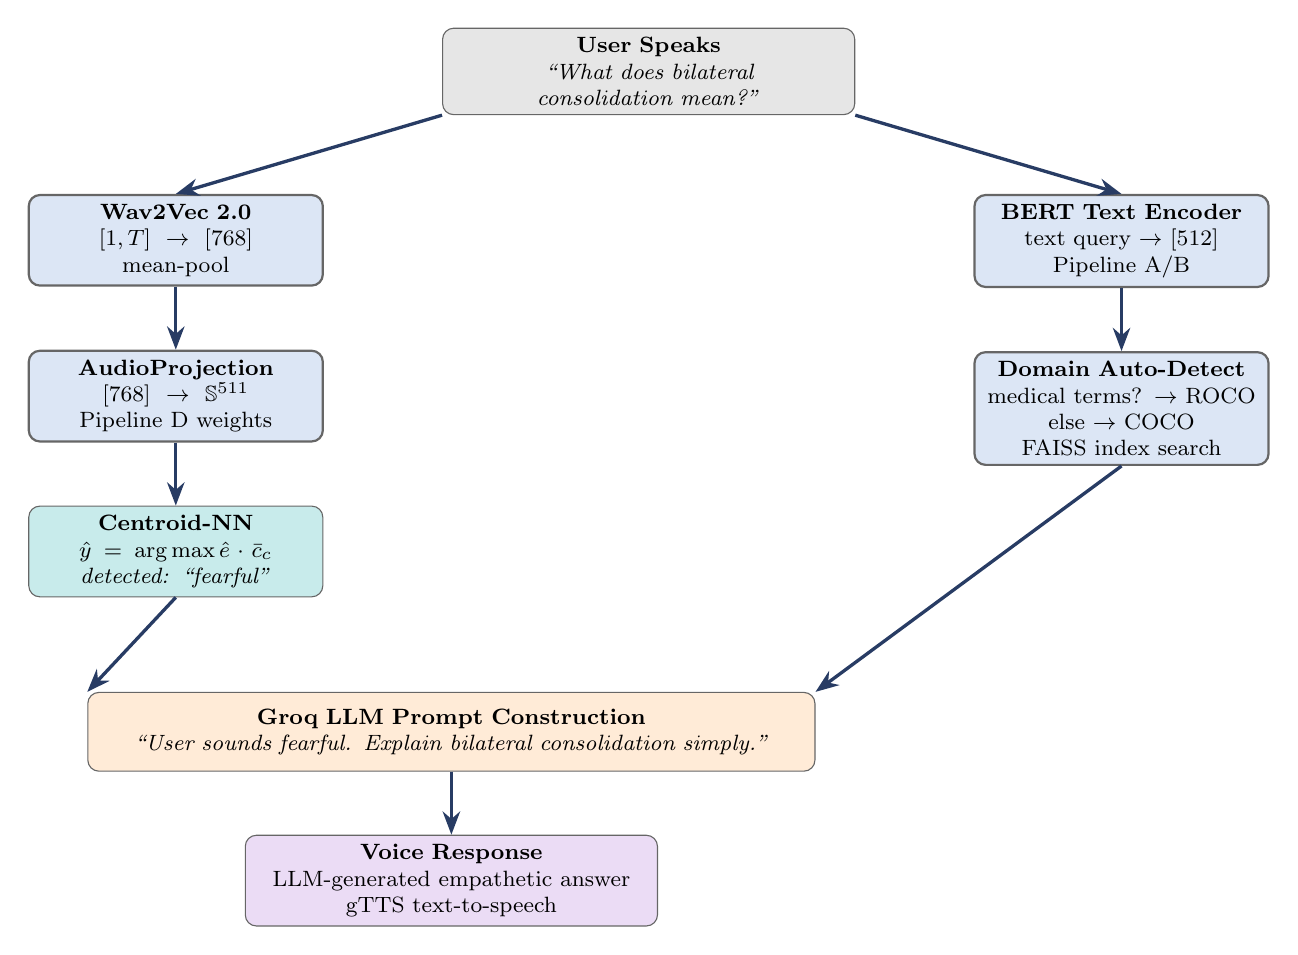
\begin{tikzpicture}[node distance=0.8cm and 1.2cm]

  \node[datanode, text width=5cm] (user)
      {\textbf{User Speaks}\\\textit{``What does bilateral consolidation mean?''}};

  % ── Split ──
  \node[pipenode, text width=3.5cm, below left=1cm and 1.5cm of user] (wav)
      {\textbf{Wav2Vec 2.0}\\$[1, T] \to [768]$\\mean-pool};

  \node[pipenode, text width=3.5cm, below right=1cm and 1.5cm of user] (bert)
      {\textbf{BERT Text Encoder}\\text query $\to$ $[512]$\\Pipeline A/B};

  \node[pipenode, text width=3.5cm, below=0.8cm of wav] (audioproj2)
      {\textbf{AudioProjection}\\$[768] \to \mathbb{S}^{511}$\\Pipeline D weights};

  \node[infernode, text width=3.5cm, below=0.8cm of audioproj2] (centroid_nn)
      {\textbf{Centroid-NN}\\$\hat{y} = \arg\max \hat{e}\cdot\bar{c}_c$\\
       \textit{detected: ``fearful''}};

  \node[pipenode, text width=3.5cm, below=0.8cm of bert] (domain)
      {\textbf{Domain Auto-Detect}\\medical terms? $\to$ ROCO\\else $\to$ COCO\\FAISS index search};

  \node[lossnode, text width=9cm, below=1.2cm of centroid_nn, xshift=3.5cm] (prompt)
      {\textbf{Groq LLM Prompt Construction}\\
       \textit{``User sounds fearful. Explain bilateral consolidation simply.''}};

  \node[outputnode, text width=5cm, below=0.8cm of prompt] (response)
      {\textbf{Voice Response}\\LLM-generated empathetic answer\\gTTS text-to-speech};

  \draw[thickarrow] (user.south west) -- (wav.north);
  \draw[thickarrow] (user.south east) -- (bert.north);
  \draw[thickarrow] (wav.south) -- (audioproj2.north);
  \draw[thickarrow] (audioproj2.south) -- (centroid_nn.north);
  \draw[thickarrow] (bert.south) -- (domain.north);
  \draw[thickarrow] (centroid_nn.south) -- (prompt.north west);
  \draw[thickarrow] (domain.south) -- (prompt.north east);
  \draw[thickarrow] (prompt.south) -- (response.north);

\end{tikzpicture}
\caption{MIVA-KNIGHT end-to-end inference flow using all four pipeline outputs.}
\label{fig:inference_flow}
\end{figure}

% ═══════════════════════════════════════════════════
\section{Output Artifacts and Reproducibility}
% ═══════════════════════════════════════════════════

\begin{table}[H]
\centering
\caption{Pipeline D saved output files}
\begin{tabularx}{\textwidth}{llXl}
\toprule
File & Format & Contents & Used by \\
\midrule
\texttt{audio\_projection\_cremad.pth} & PyTorch dict & AudioProjection weights, metadata & \texttt{pipeline.py} \\
\texttt{video\_frame\_projection.pth}  & PyTorch dict & VideoFrameProjection + ResNet state & Future work \\
\texttt{emotion\_centroids\_cremad.pt} & Tensor $[6,512]$ & Spherical centroids per emotion & Inference \\
\texttt{checkpoint\_pipelineD\_latest.pth} & Full state & Weights + optimiser + history & Resume training \\
\texttt{config.json}                   & JSON & All hyperparameters + per-emotion results & Thesis \\
\texttt{training\_curves\_pipelineD.png} & PNG & Loss + accuracy plot & Thesis \\
\bottomrule
\end{tabularx}
\end{table}

% ═══════════════════════════════════════════════════
\section{Pending Fixes and Integration Requirements}
% ═══════════════════════════════════════════════════

\begin{table}[H]
\centering
\caption{Four critical fixes required before Month 6 evaluation}
\begin{tabularx}{\textwidth}{clXl}
\toprule
\# & File & Change Required & Reason \\
\midrule
1 & \texttt{domain\_config.py} & \texttt{audio\_weights} $\to$
    \texttt{pipelineC/audio\_projection.pth} & Correct checkpoint path \\
2 & \texttt{domain\_config.py} & \texttt{emotion\_centroids} $\to$
    \texttt{pipelineC/emotion\_centroids.pt} & Correct centroids path \\
3 & \texttt{pipeline.py} & \texttt{AudioProjection(wav2vec\_dim=768)}
    (was 512) & Bug fix from Month 2 \\
4 & \texttt{encoders.py} & Verify live Wav2Vec outputs 768-d & Dimension mismatch guard \\
\bottomrule
\end{tabularx}
\end{table}

% ═══════════════════════════════════════════════════
\section{MIVA-KNIGHT 4-Pipeline Architecture Summary}
% ═══════════════════════════════════════════════════

\begin{figure}[H]
\centering
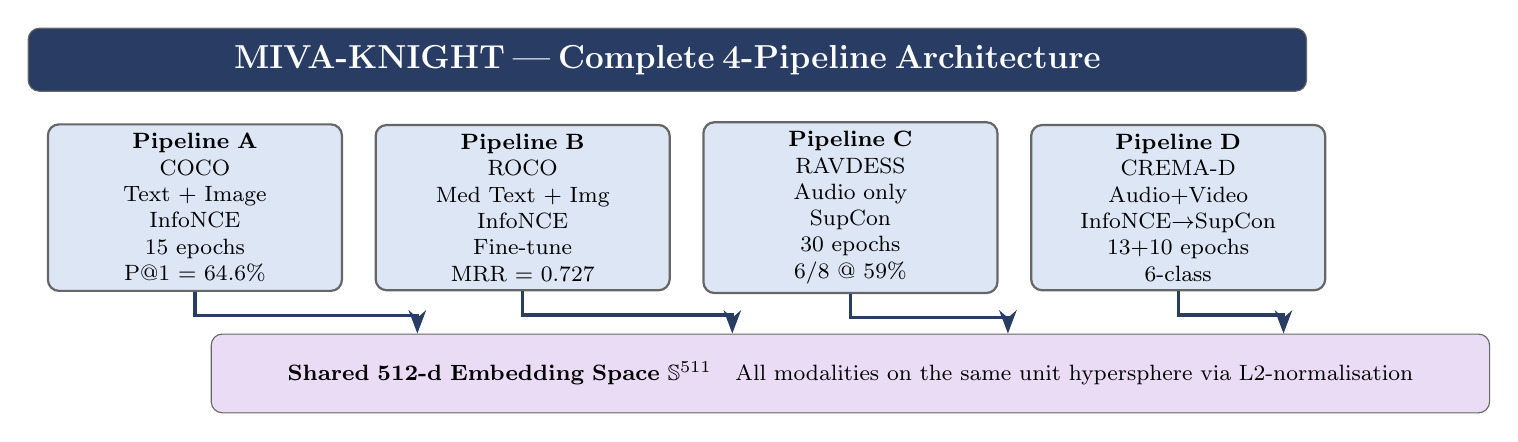
\begin{tikzpicture}[node distance=0.5cm and 0.3cm]

  % Header
  \node[basebox, fill=cDark, text=white, text width=16cm, minimum height=0.8cm] (header)
      {\large\bfseries MIVA-KNIGHT — Complete 4-Pipeline Architecture};

  % Four pipeline columns
  \node[pipenode, text width=3.5cm, below=0.4cm of header, xshift=-6.0cm] (pA)
      {\textbf{Pipeline A}\\COCO\\Text + Image\\InfoNCE\\15 epochs\\P@1 = 64.6\%};

  \node[pipenode, text width=3.5cm, right=0.4cm of pA] (pB)
      {\textbf{Pipeline B}\\ROCO\\Med Text + Img\\InfoNCE\\Fine-tune\\MRR = 0.727};

  \node[pipenode, text width=3.5cm, right=0.4cm of pB] (pC)
      {\textbf{Pipeline C}\\RAVDESS\\Audio only\\SupCon\\30 epochs\\6/8 @ 59\%};

  \node[pipenode, text width=3.5cm, right=0.4cm of pC] (pD)
      {\textbf{Pipeline D}\\CREMA-D\\Audio+Video\\InfoNCE$\to$SupCon\\13+10 epochs\\6-class};

  % Shared space node
  \node[outputnode, text width=16cm, minimum height=1.0cm, below=0.5cm of pC, xshift=0cm] (shared)
      {\textbf{Shared 512-d Embedding Space} $\mathbb{S}^{511}$\quad
       All modalities on the same unit hypersphere via L2-normalisation};

  \draw[thickarrow] (pA.south) -- ++(0,-0.3) -| ($(shared.north)+(-5.5,0)$);
  \draw[thickarrow] (pB.south) -- ++(0,-0.3) -| ($(shared.north)+(-1.5,0)$);
  \draw[thickarrow] (pC.south) -- ++(0,-0.3) -| ($(shared.north)+(2.0,0)$);
  \draw[thickarrow] (pD.south) -- ++(0,-0.3) -| ($(shared.north)+(5.5,0)$);

\end{tikzpicture}
\caption{All four MIVA-KNIGHT pipelines converging on the shared 512-d embedding space.}
\label{fig:4pipeline}
\end{figure}

% ═══════════════════════════════════════════════════
\section{Theoretical Summary: Key Results}
% ═══════════════════════════════════════════════════

\begin{theorem}[Transfer Learning Efficiency — Frozen Backbones]
Freezing both Wav2Vec 2.0 (94 M params) and ResNet-50 (23 M params) provides:
\begin{enumerate}
  \item VRAM saving: 94 M float32 $\approx$ 360 MB; freed after caching.
  \item Prevention of catastrophic forgetting of 960-hour LibriSpeech and
        ImageNet representations.
  \item Training speed-up of approximately $10\times$ per epoch (no backbone backprop).
\end{enumerate}
\end{theorem}

\begin{theorem}[Reproducible Training]
Setting \texttt{torch.manual\_seed(42)} and \texttt{np.random.seed(42)}
before any stochastic operation guarantees bit-identical results across runs
on the same hardware, assuming no non-deterministic CUDA kernels are triggered.
\end{theorem}

\begin{lemma}[Best-Epoch Selection]
Let $\text{acc}(e)$ be the centroid-NN accuracy at epoch $e$.
The selected model $\theta^* = \theta_{\hat{e}}$ where
$\hat{e} = \arg\max_e \text{acc}(e)$ minimises the expected error
of the Voronoi centroid classifier on the CREMA-D training distribution.
Accuracy is preferred over loss as the selection criterion because
the downstream use case (emotion detection in live voice queries) is
directly measured by classification accuracy, not by InfoNCE loss value.
\end{lemma}

\begin{axiom}[Unit Hypersphere Metric]
For cosine similarity to be a valid comparison metric across modalities,
all embeddings must satisfy $\|\hat{e}\|_2 = 1$. The L2-normalisation
at the end of both projection heads enforces this axiom by construction.
\end{axiom}

% ═══════════════════════════════════════════════════
\appendix
\section{Hyperparameter Reference}
% ═══════════════════════════════════════════════════

\begin{table}[H]
\centering
\caption{Pipeline D complete hyperparameter table}
\begin{tabularx}{\textwidth}{llXl}
\toprule
Hyperparameter & Value & Rationale & Shared? \\
\midrule
\texttt{EMBED\_DIM} & 512 & Shared across all 4 pipelines & All \\
\texttt{WAV2VEC\_DIM} & 768 & Wav2Vec 2.0 base output (bug-fixed from 512) & C, D \\
\texttt{RESNET\_DIM} & 2048 & ResNet-50 pool5 feature dimension & D only \\
\texttt{NUM\_EPOCHS} & 13 & $\approx$3 min/epoch $\times$ 13 = 40 min in one Colab session & D \\
\texttt{BATCH\_SIZE} & 32 & 31 negatives per InfoNCE step; fits T4 VRAM & D \\
\texttt{TEMPERATURE} & 0.07 & Sharp softmax; consistent with Pipelines A–C & A–D \\
\texttt{LEARNING\_RATE} & $10^{-4}$ & Default; $5\times10^{-5}$ on warm-start & D \\
\texttt{WEIGHT\_DECAY} & 0.01 & AdamW decoupled L2 & D \\
\texttt{SUPCON\_LR} & $10^{-5}$ & Conservative; preserves InfoNCE geometry & D (Stage 2) \\
\texttt{SUPCON\_EPOCHS} & 10 & Short refinement pass & D (Stage 2) \\
\bottomrule
\end{tabularx}
\end{table}

\section{GELU Activation Function}

\begin{definition}[GELU — Gaussian Error Linear Unit]
\[
  \text{GELU}(x) = x \cdot \Phi(x) = x \cdot \frac{1}{2}\left[1 + \text{erf}\!\left(\frac{x}{\sqrt{2}}\right)\right]
\]
where $\Phi$ is the standard normal CDF. GELU is preferred over ReLU in
transformer-adjacent architectures because it provides a smooth, stochastic
approximation of gating and tends to train faster on embedding-learning tasks.
\end{definition}

\section{LayerNorm}

\begin{definition}[Layer Normalisation]
For an input vector $h \in \mathbb{R}^d$:
\[
  \text{LN}(h) = \gamma \odot \frac{h - \mu_h}{\sqrt{\sigma_h^2 + \epsilon}} + \beta
\]
where $\mu_h = \frac{1}{d}\sum_i h_i$, $\sigma_h^2 = \frac{1}{d}\sum_i (h_i - \mu_h)^2$,
$\epsilon = 10^{-5}$, and $\gamma, \beta \in \mathbb{R}^d$ are learned scale and shift.
LayerNorm stabilises training by normalising the distribution of activations
within each sample — critical before L2-normalisation to prevent numerical issues.
\end{definition}

\end{document}
